\graphicspath{ {./bilder/} }

\subsection{Rotasjon av stive legemer}

\subsubsection{Rotasjonell kinematikk}
Når et stivt legeme roteres rundt en stasjonær akse (vanligvis $z$-aksen), så er posisjonen til det stive legemet beskrevet av vinkelen $\theta.$\newline\newline

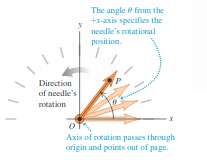
\includegraphics{rapport/metode/bilder/theta.png}\newline\newline
Her ser vi et eksempel på et stivt legeme som roterer rundt en stasjonær akse \cite{FYSIKK:1}. Som vi kan se er legemets posisjon beskrevet av $\theta.$\newline\newline
Vinkelfarten $\omega_z$ er den tidsderiverte av $\theta$, og vinkelakselerasjonen $\alpha_z$ er den tidsderiverte av $\omega_z$, eller den andrederiverte av $\theta.$
\begin{equation}
    \omega_z=\lim_{\Delta t\rightarrow0}{\frac{\Delta\theta}{\Delta t}}=\frac{d\theta}{dt}
\end{equation}
\begin{equation}
    \alpha_z=\lim_{\Delta t\rightarrow0}{\frac{\Delta\omega_z}{\Delta t}}=\frac{d\omega_z}{dt}
\end{equation}
Hvis vinkelakselerasjonen er konstant, så er $\theta$, $\omega_z$, og $\alpha_z$ relatert med kinematikk-ligningene som er ekvivalente med de som gjelder for lineær kinematikk:
\begin{equation}
    \theta=\theta_0+\omega_{0z}t+\frac{1}{2}\alpha_zt^2
\end{equation}
\begin{equation}
    \theta-\theta_0=\frac{1}{2}\left(\omega_{0z}+\omega_z\right)^2
\end{equation}
\begin{equation}
    \omega_z=\omega_{0z}+\alpha_zt
\end{equation}
\begin{equation}
    \omega_z^2=\omega_{0z}^2+2\alpha_z(\theta-\theta_0)
\end{equation}

\subsubsection{Forholdet mellom lineær og rotasjonell kinematikk}
For både lineær kinematikk og rotasjonell kinematikk gjelder følgende:\newline\newline
\begin{itemize}
    \item Vinkelhastigheten $\omega$ til et stivt legeme er lengden til vinkelfarten.
    \item Endringsraten til $\omega$ er $\alpha=\frac{d\omega}{dt}.$
    \item For en partikkel i legemet en distanse $r$ fra rotasjonsaksen, er farten og komponentene til $\vec{a}$ relatert til $\omega$ og $\alpha$ på følgende måte:
\end{itemize}
\begin{equation}
    v=r\omega
\end{equation}
\begin{equation}
    a_{\text{tan}}=\frac{dv}{dt}=r\frac{d\omega}{dt}=r\alpha
\end{equation}
\begin{equation}
    a_{\text{rad}}=\frac{v^2}{r}=\omega^2r
\end{equation}
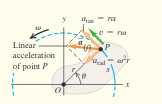
\includegraphics{rapport/metode/bilder/tang.png}\newline
Her er $a_\text{rad}$ og $a_\text{rad}$ henholdsvis den radielle komponenten og den tangentielle komponenten til akseleasjonsvektoren \cite{FYSIKK:1}

\subsubsection{Treghetsmoment og rotasjonell kinetisk energi}
Treghetsmomentet $I$ til et legeme om en gitt akse er et mål på legemets rotasjonelle treget: Jo større verdien til $I$ er, jo vanskeligere er det å endre tilstanden til rotasjonen. Treghetsmomentet kan bli skrevet som en sum over massen til partiklene, $m_i$, som utgjør hele legemet. Hver partikkel har en distanse $r_i$ fra aksen.
\begin{equation}
    I=m_1r_1^2+m_2r_2^2+\dots=\sum_i{m_i_r_i^2}
\end{equation}
Den rotasjonelle 